\chapter{DFR-FastMOT: Detection Failure Resistant Tracker for Fast  Multi-Object Tracking Based on Sensor Fusion(ICRA2023)\cite{10160328}}

\section{解决问题}
文章主要针对目标追踪中的遮挡问题做了许多工作。
非学习算法往往只保存一小段的轨迹,因此难以应对长时间的遮挡情况。
文章设计了一种代数的数据关联公式从而降低了需要计算复杂度,从而可以处理更长时间的轨迹。

\section{解决算法}
\begin{figure}[htbp]
	\centering
	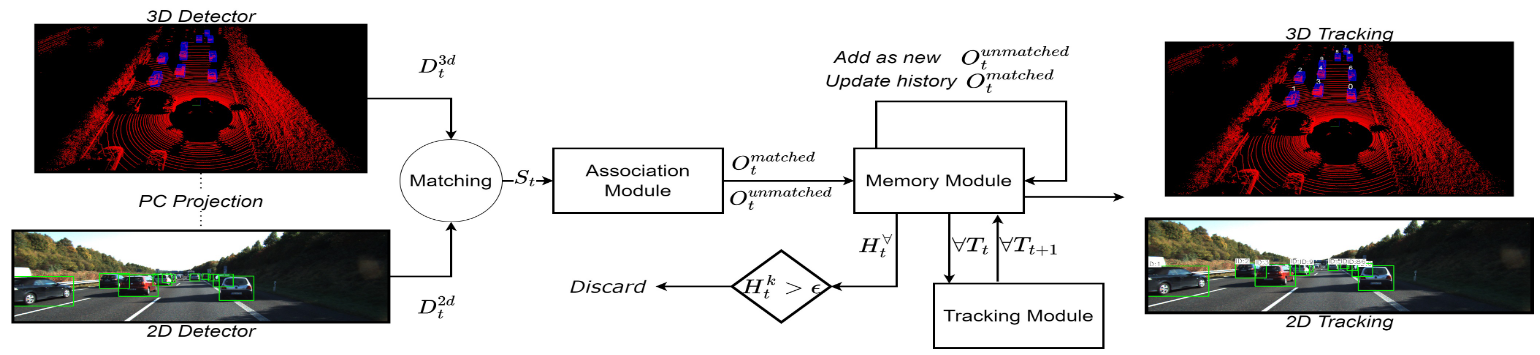
\includegraphics[width=\textwidth]{images/DFRMOT/framework.png}
	\caption{整体框架}
	\label{framework}
\end{figure}

\subsection{关联矩阵的引入}
为了提高计算的效率,文章为每种传感器设计了一个关联矩阵,矩阵的每个元素代表前一时刻对象(轨迹)的估计值和当前时刻检测值的关联程度。

\begin{figure}[H]
	\centering
	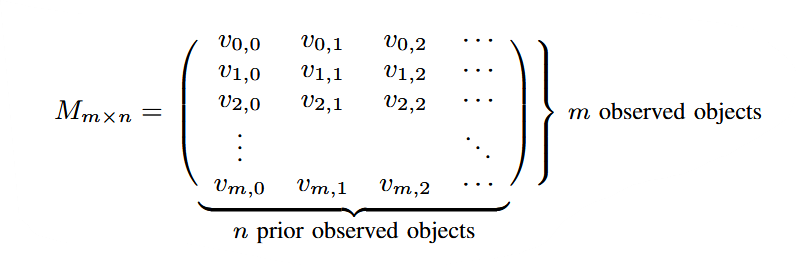
\includegraphics[width=0.8\textwidth]{images/DFRMOT/matrix.png}
\end{figure}

\begin{tcolorbox}[]

\hspace{22pt}$v_{i,j}$代表关联值,公式\ref{equ_0}处理2D情况,记作$M_c$。公式\ref{equ_1}处理3D情况,记作$M_l$。公式\ref{equ_2}将两种情况进行统一,记作$M_f$。

\begin{equation}\label{equ_0}
	v_{ij} = 
	\begin{cases}
		v_{IoU}&:v_{IoU}\leq a_c\\
		0&:\text{Otherwise}.
	\end{cases}
\end{equation}

\begin{equation}\label{equ_1}
	v_{ij} = 
	\begin{cases}
		v_{dist} & :v_{dist} < a_l\\
		a_l & :\text{Otherwise}.
	\end{cases}
\end{equation}

\begin{equation} \label{equ_2}
\begin{cases}
	M_f &= \alpha_c M_c + \alpha (1 - M_t), \\
	\alpha_c + \alpha_l &= 1, \\
	\alpha_c , \alpha_l &\leq 1.
\end{cases}
\end{equation}

\hspace{22pt}得到所有关联矩阵之后,便可以进行数据关联。文章采用了类匈牙利算法来实现该步骤。
最后所有的计算复杂度为:
$$ \mathcal{O}(2mn) \rightarrow \mathcal{O}(m^2n^2) \rightarrow \mathcal{O}(m^2n^2) $$

\end{tcolorbox}

\subsection{其它处理方法}
1. 3D距离函数的选用

为了处理遮挡的情况,文章采用了3D中心距离来衡量两个目标的相似程度,而不是传统的IoU。当出现长时间的遮挡情况时,去计算IoU是十分困难的,而计算3D的距离则更容易实现。

2. KF计算简化

在用KF计算目标下一时刻的状态时,需要进行大量的矩阵运算。为此,作者采用最少点数来描述目标位置:2D两个,3D两个。

\section{文章结果}
文章通过使用不同质量的检测器来模拟遮挡的效果。结果表明,文章显著提高了低质量检测器的追踪效果。整体而言,追踪的精度也有所提高。
\begin{figure}
	\centering
	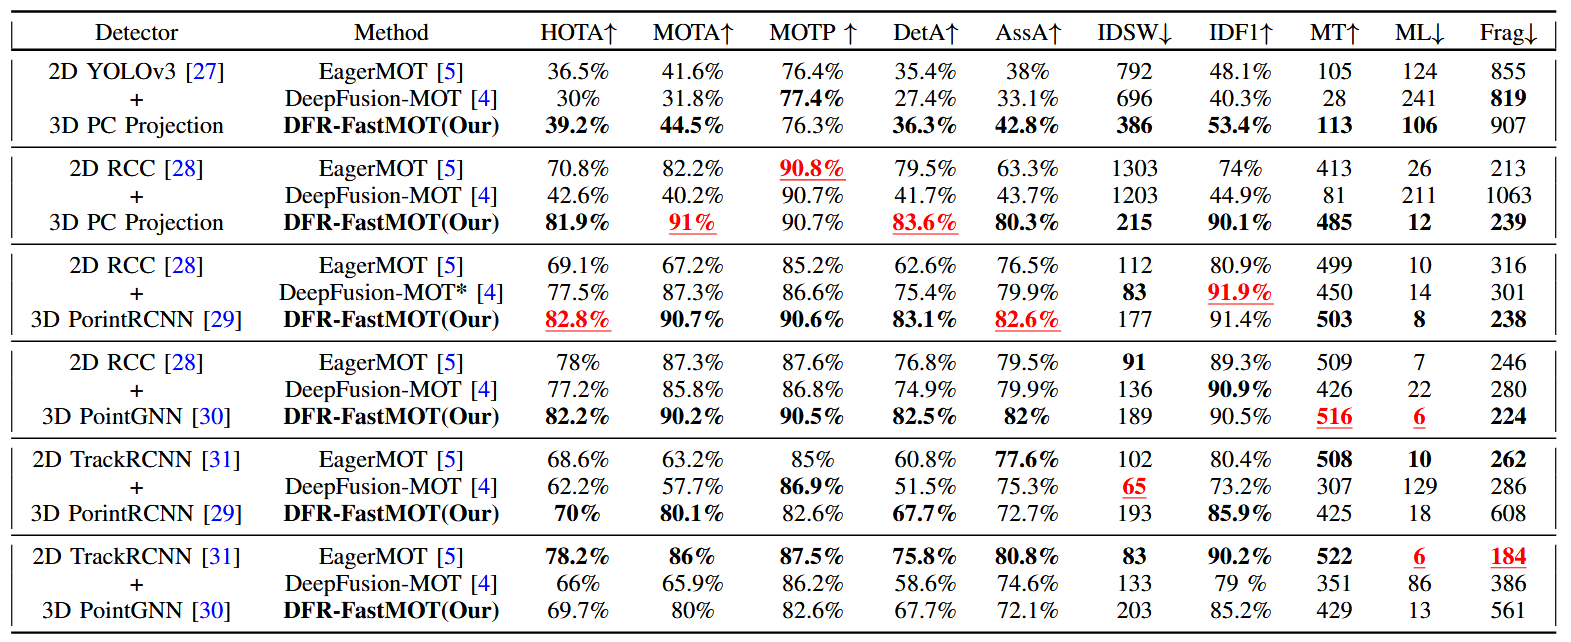
\includegraphics[width=\textwidth]{images/DFRMOT/result.png}
\end{figure}


\section{学习总结}
DFRMOT也是采用DBT追踪框架,具体内容也基本和EagerMOT相似。其主要工作在于提出了一种提高计算效率的关联矩阵,由此多出的冗余可以用来计算更长时间的目标,间接的提高了应对遮挡的能力。

所以,在自己设计的追踪器上,就可以采用本文设计的关联矩阵提高计算效率。
此外,本外还在细节上提出了许多加速方法,我们可以直接应用他的计算框架来完成更复杂的任务。